%%%%%%%%%%%%%%%%%%%%%%%%%%%%%%%%%%%%%%%%%
% Thin Sectioned Essay
% LaTeX Template
% Version 1.0 (3/8/13)
%
% This template has been downloaded from:
% http://www.LaTeXTemplates.com
%
% Original Author:
% Nicolas Diaz (nsdiaz@uc.cl) with extensive modifications by:
% Vel (vel@latextemplates.com)
%
% License:
% CC BY-NC-SA 3.0 (http://creativecommons.org/licenses/by-nc-sa/3.0/)
%
%%%%%%%%%%%%%%%%%%%%%%%%%%%%%%%%%%%%%%%%%

%----------------------------------------------------------------------------------------
%	PACKAGES AND OTHER DOCUMENT CONFIGURATIONS
%----------------------------------------------------------------------------------------

\documentclass[a4paper, 11pt]{article} % Font size (can be 10pt, 11pt or 12pt) and paper size (remove a4paper for US letter paper)

\usepackage[protrusion=true,expansion=true]{microtype}	% Better typography
\usepackage{graphicx} 		% Required for including pictures
\usepackage{wrapfig}  		% Allows in-line images
\usepackage{hyperref}		% Allows the use of hyperlinks
\usepackage{amsmath}
\usepackage{multirow}

\usepackage{mathpazo}		% Use the Palatino font
\usepackage[T1]{fontenc} 	% Required for accented characters
\usepackage[utf8]{inputenc}     % Spanish characters
\usepackage{amsmath} 		% Allows align
\usepackage{listings}		% Allows code 
\usepackage{subfig}


\linespread{1.05} % Change line spacing here, Palatino benefits from a slight increase by default

\makeatletter
\renewcommand\@biblabel[1]{\textbf{#1.}} % Change the square brackets for each bibliography item from '[1]' to '1.'
\renewcommand{\@listI}{\itemsep=0pt} % Reduce the space between items in the itemize and enumerate environments and the bibliography

\renewcommand{\maketitle}{ % Customize the title - do not edit title and author name here, see the TITLE block below
\begin{flushright} % Right align
{\LARGE\@title} % Increase the font size of the title

\vspace{50pt} % Some vertical space between the title and author name

{\large\@author} % Author name
\\\@date % Date

\vspace{40pt} % Some vertical space between the author block and abstract
\end{flushright}
}

%----------------------------------------------------------------------------------------
%	TITLE
%----------------------------------------------------------------------------------------

\title{\textbf{Árboles de decisión}}

\author{
	\textsc{Agustín Mista}\\
	\textit{Universidad Nacional de Rosario}\\
 	\textit{Introducción a la Inteligencia Artificial}
}

\date{Rosario, 2 de Abril de 2017}

%----------------------------------------------------------------------------------------

\begin{document}

\maketitle % Print the title section

%----------------------------------------------------------------------------------------
%	ABSTRACT
%----------------------------------------------------------------------------------------

%\renewcommand{\abstractname}{Summary} % Uncomment to change the name of the abstract to something else

%\begin{abstract}
%	Cuando todo esté cocinado, voy a completar este abstract con información pertinente.
%\end{abstract}

\vspace{20pt} % Some vertical space between the abstract and first section

%----------------------------------------------------------------------------------------
%	ESSAY BODY
%----------------------------------------------------------------------------------------

\section*{Introducción}

%\begin{wrapfigure}{o}{0.45\textwidth}
%	\begin{center}
%		\vspace{-20pt}
%		\includegraphics[width=0.4\textwidth]{lena-sample.png}
%		\vspace{-20pt}
%	\end{center}
%\end{wrapfigure}

\pagebreak

%------------------------------------------------

\section*{Apartado 4}  Genere tres conjuntos de datos de entrenamiento
correspondientes al problema de las espirales anidadas de la práctica 0, uno de
longitud 150, otro de 600 y un tercero de 3000. Genere un conjunto de test de
longitud 10000. Cree el archivo .names necesario para el problema. A partir de
cada uno de los conjuntos de entrenamiento, desarrolle el árbol de decisión
correspondiente y grafique las predicciones sobre el conjunto de test (archivo
.prediction). Comente los resultados.

\begin{figure}
  \centering
  \subfloat[Caption 1]{\label{ref_label1}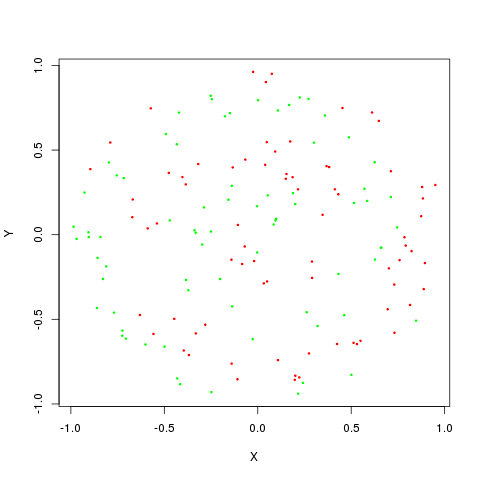
\includegraphics[width=0.5\textwidth]{../datasets/spiral/spiral150.data.png}}
  \subfloat[Caption 1]{\label{ref_label1}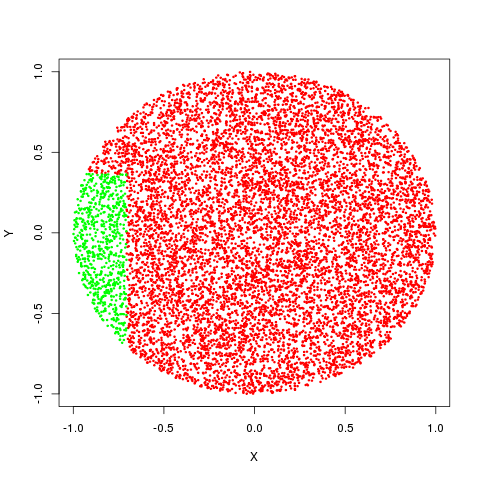
\includegraphics[width=0.5\textwidth]{../datasets/spiral/spiral150.prediction.png}}
  \caption{\label{ref_label_overall}Overall caption}
\end{figure}

\end{document}
